\newpage
\section{ПРАКТИЧЕСКАЯ ЧАСТЬ}

В основе пакета компьютерного моделирования лежат следующие программные \mbox{блоки}:
\begin{itemize}
    \item \textbf{базовые математические функции,} используемые для работы с матрицами и векторами, для расчёта положения объектов в трёхмерном пространстве, для решения функций минимизации;
    \item \textbf{программное представление кинематической структуры ПМР;}
    \item \textbf{решение ОЗК} для нахождения вариантов пространственной конфигурации звеньев ПМР при достижении точки в пространстве;
    \item \textbf{средства отображения трёхмерной графики;}
    \item \textbf{пользовательский интерфейс на основе оконного приложения.}
\end{itemize}


\subsection{\textbf{Реализация базовых математических функций}}

Для реализации кинематической схемы моделируемого промышленного робота необходимо использование методов линейной алгебры, векторной геометрии и матричных уравнений при расчёте положений звеньев манипулятора. Для использования перечисленных математических функций требуется использование сторонних математических библиотек, а также написания собственных расчётных функций.

\subsubsection{\textbf{Использованные внешние библиотеки}}

В качестве библиотеки для линейной алгебры, векторных и матричных вычислений используется C++ библиотека Eigen\cite{Eigen_Lib}.

\textbf{Eigen} -- библиотека линейной алгебры для языка программирования C++ с открытым исходным кодом. Написана на шаблонах и предназначена для векторно-матричных вычислений и связанных с ними операций.

Eigen не имеет никаких зависимостей, кроме стандартной библиотеки C++ и использует систему сборки CMake, поддерживает множество компиляторов C++.

Eigen -- библиотека с открытым исходным кодом, бесплатно распространяющаяся для ознакомительных, учебных и коммерческих целей. 

Из библиотеки функций Eigen используются:
\begin{itemize}
    \item поддержку комплексных чисел в вычислениях;
    \item структура "вектор", поддерживающая векторы динамического размера и математические операции над ними;
    \item шаблон универсальной матрицы, подходящий для многомерных вычислений. 
\end{itemize}

\newpage
\subsubsection{\textbf{Реализованные математические функции}}

При решении поставленной задачи были реализованы следующие математические функции:

\begin{itemize}
    \item 
Функции \textbf{DegToRad} и \textbf{RadToDeg} для перевода значений угла из градусов в радианы и обратно. В качестве аргумента и вывода функции используется тип числа с плавающей точкой.
\item
Функция вычисления проекции одного вектора на другой \textbf{projVector}.
\begin{equation} \label{eq_projVec}
    % \vec{}
    l = \frac{\bar{a} \cdot \bar{b}}{\left |\bar{b} \right|} % уравнение
\end{equation}

В качестве аргументов $\bar{a}$ и $\bar{b}$ уравнения \eqref{eq_projVec} принимаются два трёхмерных вектора, а выводится длина $l$ проекции в миллиметрах в виде числа с плавающей точкой. Функция может обрабатывать исключение и выдавать ошибку при подстановки в $\bar{b}$ нулевого вектора.

~

\item
Функция вычисления угла между векторами \textbf{getAngle}.
\begin{equation} \label{eq_getAngle}
    % \vec{}
    \alpha = \arccos{\frac{\bar{a} \cdot \bar{b}}{\left |\bar{a} \right| \cdot \left |\bar{b} \right|}} % уравнение
\end{equation}

В качестве аргументов $\bar{a}$ и $\bar{b}$ уравнения \eqref{eq_getAngle} принимаются два трёхмерных вектора, а выводится угол $\alpha$ между векторами в радианах в виде числа с плавающей точкой. Функция может обрабатывать исключение и выдавать ошибку при подстановки в $\bar{a}$ или $\bar{b}$ нулевого вектора.

~

\item
Функция вычисления угла между векторами с учётом направления вращения вокруг заданной оси \textbf{getAngleAroundAxis}.

На первом шаге вычисляются новые вектора $\bar{a_1}$ и $\bar{b_1}$, являющиеся проекциями векторов на плоскость перпендикулярную оси $\bar{Axis}$

Дальше вычисляется угол между двумя проекциями:
\begin{equation} \label{eq_getAngleAroundAxis}
    % \vec{}
    \alpha = \arccos{\frac{\bar{a_1} \cdot \bar{b_1}}{\left |\bar{a_1} \right| \cdot \left |\bar{b_1} \right|}} % уравнение
\end{equation}

Последним шагом вычисляется векторное произведение $\bar{c} = \bar{a_1} \times \bar{b_1}$, по направлению которого относительно $\bar{Axis}$ определяется знак ответа.

В качестве аргументов $\bar{a}$, $\bar{b}$ и $\bar{Axis}$ уравнения \eqref{eq_getAngleAroundAxis} принимаются три трёхмерных вектора -- два вектора для сравнения и ось поворота, а выводится угол $\alpha$ с учётом знака в радианах в виде числа с плавающей точкой. Функция может обрабатывать исключение и выдавать ошибку при подстановки в $\bar{a}$, $\bar{b}$ или $\bar{Axis}$ нулевого вектора, а также при подстановки векторов, параллельных оси $\bar{Axis}$.

\item 
Функции \textbf{Rx}, \textbf{Ry} и \textbf{Rz} для получения матриц поворота относительно осей \textbf{X}, \textbf{Y} и \textbf{Z} соответственно. В качестве аргумента функции используется $\alpha$ -- угол поворота вокруг оси используя тип числа с плавающей точкой.

\begin{equation}
Rx =
\begin{pmatrix}
1 & 0 & 0\\
0 & \cos{\alpha} & -\sin{\alpha}\\
0 & \sin{\alpha} &  \cos{\alpha}
\end{pmatrix}
\end{equation}

\begin{equation}
Ry =
\begin{pmatrix}
 \cos{\alpha} & 0 & \sin{\alpha}\\
            0 & 1 & 0\\
-\sin{\alpha} & 0 & \cos{\alpha}
\end{pmatrix}
\end{equation}

\begin{equation}
Rz =
\begin{pmatrix}
\cos{\alpha} & -\sin{\alpha} & 0\\
\sin{\alpha} &  \cos{\alpha} & 0\\
0 & 0 & 1
\end{pmatrix}
\end{equation}

~

~

\item 
Функция \textbf{calcJacobian} для вычисления по данной дифференцируемой многомерной функции $Y = F(X)$ и известной функцией подсчёта ошибки, в инициирующей точке $X_0$, с заданной точностью $e$.

\begin{equation}
J = \left(
\begin{array}{cccc}\label{Jac}
\frac{\partial y_1}{\partial x_1} & \frac{\partial y_1}{\partial x_2} & \ldots & \frac{\partial y_1}{\partial x_n}\\
\frac{\partial y_2}{\partial x_1} & \frac{\partial y_2}{\partial x_2} & \ldots & \frac{\partial y_2}{\partial x_n}\\
\vdots & \vdots & \ddots & \vdots\\
\frac{\partial y_n}{\partial x_1} & \frac{\partial y_n}{\partial x_2} & \ldots & \frac{\partial y_n}{\partial x_n}
\end{array}
\right)
\end{equation}

Для вычисления Якобиана функции $(y_1, y_2,...,y_n) =  f(x_1, x_2,...,x_n)$ необходимо найти частные производные всех $y_i$ системы по всем переменным $x_i$. Для этого от инициирующей точки отступается шаг по увеличению и по уменьшению одной из координат на величину заданной точности. Вычисляются и сравниваются значения функции в полученных точках, получая величину ошибки. При делении полученной разности ошибок на удвоенную точность получается частичная производная по переменной $x_i$.
\begin{equation}\label{JacCol}
J_i = \left(
\begin{array}{c}
\frac{\partial y_1}{\partial x_i}\\
\frac{\partial y_2}{\partial x_i}\\
\vdots\\
\frac{\partial y_n}{\partial x_i}
\end{array}
\right)
\end{equation}

После прохождения $i$ по всему отрезку от $1$ до $n$ из полученных столбцов $J_i$ (\ref{JacCol}) строится матрица $J$ (\ref{Jac}).

~

\newpage
\item 
Функция \textbf{BFGS} реализация алгоритма Бройдена -- Флетчера -- Гольдфарба -- Шанно.

На вход функции подаётся точка поиска, количество независимых аргументов системы, дифференцируемая функция, функция оценки спуска и её производная, начальное приближение, дополнительно можно задать точность, величину шага изменения, максимальное количество итераций для поиска. 

Порядок работы:

\begin{enumerate}
\item \textbf{Инициализация}: Задаётся начальное приближение матрицы Гессиана $H_0$ как единичная матрица.

\item \textbf{Получение направления поиска}: Решается система $H_k \cdot p = -g_k$ для получения направления поиска $p$, где $H_k$ - текущая аппроксимация матрицы Гессиана, а $g_k$ - градиент функции в точке $x_k$.

\item \textbf{Одномерная оптимизация (поиск по линии)}: Находится приемлемый размер шага $\alpha_k$ в направлении $p$, полученном на предыдущем шаге.

\item \textbf{Обновление}: Вычисляется новая точка $x_{k+1} = x_k + \alpha_k p$.

\item \textbf{Обновление Гессиана}: Обновляется аппроксимация матрицы Гессиана $H_k$ на основе градиента в новой точке и разности градиентов.

\item \textbf{Проверка условий остановки}: Если выполнены условия остановки (например, $||g_k|| < \varepsilon$ для некоторого малого $\varepsilon > 0$), алгоритм останавливается. В противном случае начинаем с шага 2.
\end{enumerate}

\end{itemize}

~

~

Реализация данных программных методов приведена в приложении 1 и 2.

\newpage
\subsection{\textbf{Реализация математических зависимостей манипулятора}}

В качестве способа хранения кинематических и инерционных параметров ПМР используется C++ класс RobotArm, реализованный в файлах RobotArm.h и RobotArm.cpp (Приложение 9 и 10).

Внутри класса реализованы динамические массивы звеньев робота и его сочленений, созданы метода добавления звеньев и степеней подвижности между ними с последующей реинициализацией параметров рассматриваемой модели ПМР, а также функции решения ПЗК и ОЗК.

Для хранения характеристик звеньев и сочленений создаются классы RobotLink (Приложение 7 и 8 -- RobotLink.h, RobotLink.cpp) RobotJoint (Приложение 5 и 6 -- RobotJoint.h, RobotJoint.cpp).

Для согласования взаимодействия классов и добавления общих \hspace{0,1cm}функций \hspace{0,1cm}подсчета  \mbox{создаётся }библиотека функций RobotAdditions  (Приложение 3 и 4 \hspace{0,4cm}--\hspace{0,4cm} RobotAdditions.h, RobotAdditions.cpp).

\subsubsection{\textbf{Определение параметров Денавита–Хартенберга}}

Для решения ПЗК манипулятора требуется получить матрицу перехода для TCP относительно основания робота. Данное преобразование легко выполнить, используя параметры Денавита — Хартенберга.

Вычисление параметров Денавита — Хартенберга каждого звена ПМР происходит по следующему алгоритму:

\begin{enumerate} [label = \arabic*)]
    \item определение точек отсчета параметров из конфигурации звеньев ПМР;
        \begin{gostfigure} % Рамки для счётчика рисунков
    \begin{figure}[h] % Рамки для отрисовки
        \centering % Центрирование
        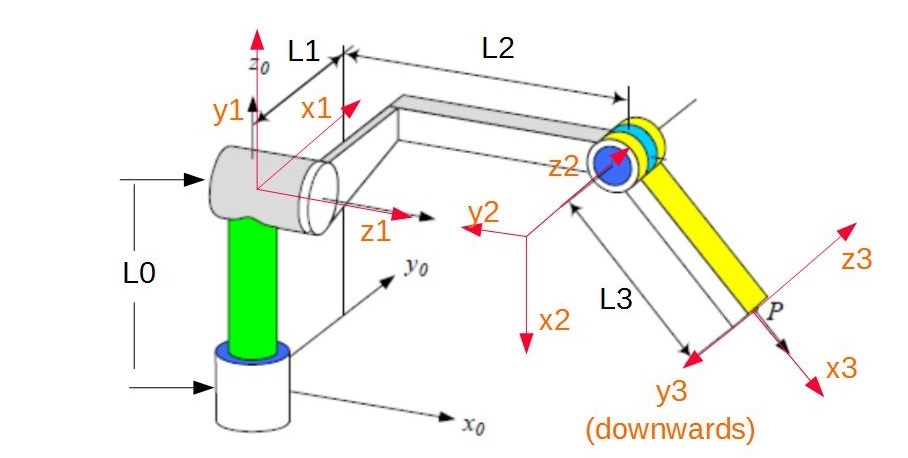
\includegraphics[width=100mm]{DH_Params.jpg} % Файл изображения
        \caption{Пример определения точек отсчёта параметров Денавита — Хартенберга} % Подпись к изображению
    \end{figure}
\end{gostfigure}
    \item расчет параметров, используя соотношение:
    \begin{itemize}
        \item $a_i$ - расстояние вдоль оси $x_i$ от $z_i$ до $z_i$
        \item $\alpha_i$ - угол вокруг оси $x_i$ от $z_i$ до $z_i$
        \item $d_i$ - расстояние вдоль оси $z_i$ от $x_i$ до $x_i$
        \item $\theta_i$ - угол вокруг оси $z_i$ от $x_i$ до $x_i$
\end{itemize}

\end{enumerate}

\newpage

\begin{figure}[!tbp]
  \centering
  \begin{gostfigure}
  \begin{minipage}[b]{0.4\textwidth}
    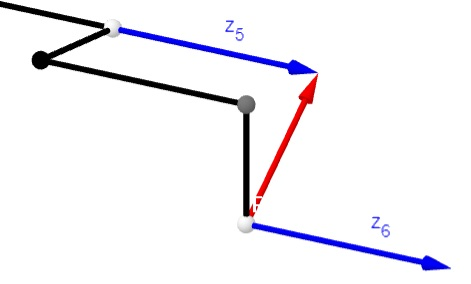
\includegraphics[width=\textwidth]{DH_Conf_P.jpg}
    \caption{Определение точки отсчёта и направления осей в параллельном случае}
    \label{img_DH_Conf_P}
  \end{minipage}
  \end{gostfigure}
  \hfill
  \begin{gostfigure}
  \begin{minipage}[b]{0.4\textwidth}
    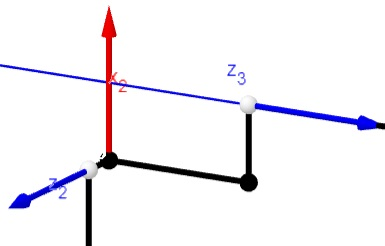
\includegraphics[width=\textwidth]{DH_Conf_NP.jpg}
    \caption{Определение точки отсчёта и направления осей в непараллельном случае}
    \label{img_DH_Conf_NP}
  \end{minipage}
  \end{gostfigure}
  
\end{figure}


Так как в рамках решаемой задачи рассматриваются ПМР, направления степеней подвижности которых параллельны осям мировой системы координат, то для определения точек отсчёта все конфигурации звеньев можно разделить на две группы: с параллельными входной и выходной осями звена и с не параллельными. Конфигурацию осей $x$ и $z$ звена относительно предыдущего можно увидеть на рисунках \ref{img_DH_Conf_P} и \ref{img_DH_Conf_NP}. Из данных о координатах полученной точки и направления осей $x$ и $z$ вычисляются параметры Денавита — Хартенберга.

~

~

\subsubsection{\textbf{Решение обратной задачи кинематики}}

Для решения ОЗК внутри класса RobotArm реализован метод \textbf{solveIK-POS}, использующий алгоритм BFGS из написанной библиотеки математики. Для работы алгоритма вовнутрь функции \textbf{MathAdditions::BFGS} передаются следующие параметры:

\begin{enumerate} [label = \arabic*)]
    \item желаемая точка положения TCP робота в пространстве в виде матрицы 4 на 4, где $R$~--~матрица поворота:
    \begin{equation}
POINT = \left(
\begin{array}{cccc}\label{point_mat}
  &   &   & x_{point} \\
  & R &   & y_{point} \\
  &   &   & z_{point} \\
0 & 0 & 0 & 1
\end{array}
\right)
\end{equation}
    \item количество степеней свободы;
    \item ссылку на метод решения ПЗК из класса RobotArm;
    \item ссылки на функции оценки спуска из библиотеки RobotAdditions;
    \item исходное положение ПМР как начальное приближение для поиска.
\end{enumerate}

В результате получаем вектор размера количества степеней свободы, элементы которого являются обобщёнными координатами каждой степени подвижности ПМР.

\newpage
\subsection{\textbf{Графическое ядро приложения}}
Для создания пользовательского интерфейса разрабатываемого программного обеспечения моделирования работы ПМР создается графическая оболочка приложения.

Её структура такова:
\begin{itemize}
    \item \textbf{уровень отрисовки трёхмерных моделей} -- основная часть пользовательского интерфейса;
    \item \textbf{уровень оконного оформления приложения} -- модуль, отвечающий за вызов средства отображения трёхмерной графики в среде ОС;
    \item \textbf{уровень отрисовки инфографики отслеживаемых показателей ПМР.}
\end{itemize}

Для каждого из этих уровней выбирается сторонняя библиотека для оптимизации процесса разработки.

\subsubsection{\textbf{Выбор средств отображения трёхмерных моделей}}

В качестве библиотеки для работы с трёхмерной графикой была выбрана библиотека BGFX.

BGFX -- кроссплатформенная, не зависящая от графического API, библиотека рендеринга с открытым исходным кодом.

\subsubsection{\textbf{Реализация пользовательского оконного интерфейса}}

В качестве библиотек для взаимодействия с оконным интерфейсом ОС были выбраны библиотеки SDL3 и ImGUI.

SDL -- Simple DirectMedia Layer -- это кроссплатформенная библиотека разработки, предназначенная для обеспечения низкоуровневого доступа к аудио, клавиатуре, мыши, джойстику и графическому оборудованию компьютера.

Immediate Mode Graphical User Interface (ImGui) -- библиотека графического интерфейса, используемая для быстрой отрисовки пользовательского интерфейса.

\subsubsection{\textbf{Вывод результатов моделирования}}

Для работы с графиками, диаграммами и другими способами визуализации данных используется библиотека Matplot++.

Matplot++ -- это графическая библиотека для визуализации данных, которая обеспечивает интерактивное построение графиков, средства для экспорта графиков в высококачественные форматы для научных публикаций, компактный синтаксис, совместимый с аналогичными библиотеками, десятки категорий графиков со специализированными алгоритмами, несколько стилей кодирования и хранения инженерных данных.